\documentclass[12pt]{cms-tdr}
\RCS$Revision: 1.0 $
\RCS$Date: Wed Sep 22 19:27:03 CDT 2010 $
\RCS$Name: Jim Pivarski $
\input{ptdr-definitions}
\cmsNoteHeader{EXO-10-999}

\newcommand{\s}[1]{{\mbox{\scriptsize #1}}}

\textheight=8.5 in

\title{Search for Collimated Groups of Muons}
\author{Jim Pivarski, Alexei Safonov, Aysen Tatarinov}
\date{\today}

\abstract{We present an inclusive, signature-based search for groups
  of collimated muons, arising from spectroscopic cascades in a hidden
  sector accessible only through high-energy collisions, using the CMS
  detector.  In several signatures defined by number of muons per
  collimated group and number of groups per event, we searched for the
  lightest state in the hidden spectrum with a mass-peak fit and set
  limits on $\sigma\mathcal{B}\alpha$, where $\alpha$ is the model
  acceptance of the signature.  Depending on the signature and the
  mass of the lightest state ($2m_\mu$--5~GeV/$c^2$), new resonances
  are ruled out at the level of $XX$-$YY$~pb for 95\% C.L.  We also
  set $\sigma\mathcal{B}$ limits on two representative benchmark
  models: SUSY dark matter with a $\mathcal{U}(1)_\s{dark}$ and NMSSM
  Higgs escaping LEP limits via Higgs-to-Higgs decays. \vspace{0.5
    cm}}

\hypersetup{%
pdfauthor={CMS Collaboration},%
pdftitle={Search for Collimated Groups of Muons},%
pdfsubject={CMS},%
pdfkeywords={CMS, physics, exotica, muons}}

\begin{document}
\maketitle

\section{Introduction}

\subsection{Motivation}

\fixme{Needs a lot of references.}

Although the dimuon mass spectrum is well understood in $e^+e^-$ and
$p\bar{p}$ collisions up to 0.2 and 2~TeV respectively, (\fixme{get
  real numbers}) new states may be hidden by weak couplings to
Standard Model particles.  A wide class of hidden-valley models
predicts new states coupling weakly to the Standard Model yet
significantly to a hidden sector, with strong mixing between the
Standard Model and the hidden sector only for massive particles.  In
these scenarios, high collision energies are necessary to create
massive particles $M$, but these particles can then decay through the
whole spectrum to the lightest hidden state: $pp \to M\overline{M}$
and $M \to m X$ where $m$ is the lightest hidden particle.  If $m$ is
unstable, it would decay with very small width to the
kinematically-accessible Standard Model states, either democratically
($Z$-like) or to the heaviest accessible state (Higgs-like).
Muon-pair final states would appear as a low-mass, high-momentum
dimuon resonance, and therefore be collimated by relativistic boost.
With several low-mass states in the decay chain, e.g.\ $m_2 \to m_1
m_1 \to 4\mu$, cascades would either produce two groups of collimated
dimuons or one group of four collimated muons, depending on the boost
of $m_2$.  Arbitrarily complex decay chains are conceivable, and
groups of muons might be produced in association with other Standard
Model pairs, such as $e^+e^-$ and $\pi\pi$.  These striking signatures
are often called ``lepton jets.''

Hidden, low-mass resonances are especially interesting in light of the
high-energy positron excess reported by the PAMELA primary cosmic-ray
experiment.  This excess of interstellar positrons could be the
product of WIMP annihilations, assuming that the WIMP annihilation
rate is higher than what would be expected from thermal freeze-out in
the early universe, and also assuming some mechanism to prohibit decay
chains that produce antiprotons, in which no excess was observed.  A
new force boson, $z_\s{dark}$, with a mass of approximately
1~GeV/$c^2$ and coupling significantly to WIMPs yet weakly to Standard
Model particles, would explain both observations.  Acting as a
long-range Yukawa force, $z_\s{dark}$ would draw together slow-moving
WIMPs, increasing their effective annihilation cross-section in the
modern era without affecting their production in the early universe.
As a decay channel, $z_\s{dark} \to p\bar{p} X$ would be
kinematically forbidden if the mass of $z_\s{dark}$ were above
2~GeV/$c^2$ or so.  Relatively simple extensions of this picture, such
as adding a dark Higgs boson $h_\s{dark}$ to give the $z_\s{dark}$ its
mass, or introducing the force with non-abelian structure, would
produce more complex event topologies: $2^N$ fermion pairs per lepton
jet for an $N$-state decay chain and/or several lepton jets per event.

Another, very different, motivation derives from the tension between
the low Higgs mass predicted by precision electroweak fits and the
direct LEP limit of 114~GeV/$c^2$.  This limit assumes that the Higgs
boson decays directly into Standard Model particles with known
branching fractions.  If additional light Higgs bosons allow for
Higgs-to-Higgs decays, the direct limit may be circumvented.  In a
well-defined region of Next-to Minimal SuperSymmetric (NMSSM)
parameter space, the lightest CP-odd Higgs ($a_1$) can have
arbitrarily low mass.  Below the $2m_\tau$ threshold, the branching
fraction for $a_1 \to \mu\mu$ is about 20\%, making its detection in
the muon channel visible.  For values of the NMSSM parameters that
give the lightest CP-even Higgs ($h_1$) a large singlet field
component, $h_1 \to a_1 a_1$ can be as large as 100\%.  If nature has
chosen this model, then the Higgs mass could be as low as 86~GeV/$c^2$
and the primary Higgs signature would be $h_1 \to a_1 a_1 \to 2\mu,
2\mu$, where the dimuons appear as well-collimated lepton jets.

\subsection{Method}

In this paper, we present an inclusive, signature-based search for
collimated dimuons with $2m_\mu < \mbox{mass} < 5$~GeV/$c^2$ arising
from hidden cascade chains.  Additional objects, such as isolated
single leptons, hadronic jets, and missing energy, are neither
included in the search nor are they forbidden.  In particular, boosted
dimuons are not rejected if they are overlapped by $e^+e^-$ or
$\pi\pi$ from other resonance decays in the same lepton jet, nor are
they rejected due to activity from a nearby hadronic jet that might
arise, for example, from SUSY cascade decays.

We assume that all decay chains in the hidden sector end with a
low-mass state $m_1$ before decaying to opposite-sign muon pairs,
though there may be several instances of this particle per event,
possibly overlapping one another.  This assumption is equivalent to
assuming that the coupling between the hidden states and the Standard
Model is much weaker than the couplings of the hidden states with each
other.  We therefore search for one new resonance with a single dimuon
mass peak, after identifying the combination of muon pairs that is
most likely to have arisen from distinct resonance decays.

Identifying the distinct dimuon resonances proceeds in two steps.
First, nearby muons are grouped into ``mu-jets'' with an arbitrary
number of muons per group.  The definition of ``nearby muons'' is
kinematic rather than geometric: two muons are considered near each
other if their pairwise invariant mass is less than 5~GeV/$c^2$ with
both muons satisfying a minimim-$p_T$ threshold.  This differs from
selections based on a maximum $\Delta R = \sqrt{(\Delta \phi)^2 +
  (\Delta \eta)^2}$ because $\Delta R$ approximately corresponds to
relativistic boost, effectively a tighter requirement on resonance
momentum for higher resonance masses (see
Fig.~\ref{fig:openingangle_dr}).

\begin{figure}
\begin{center}
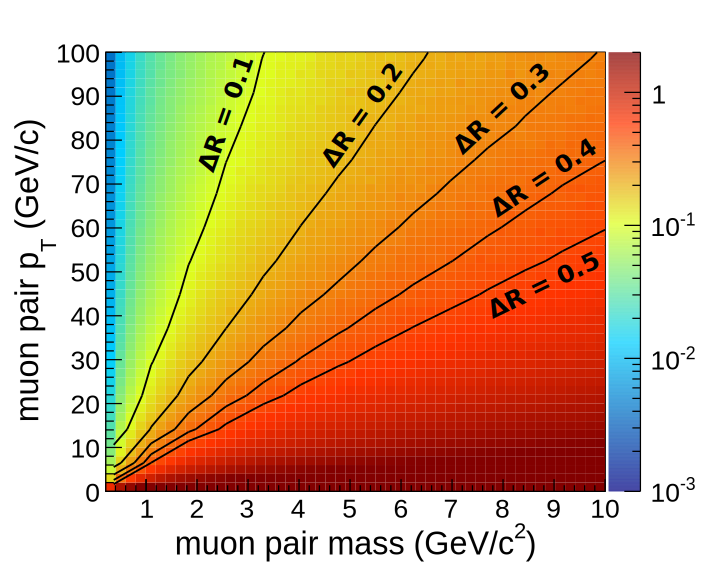
\includegraphics[width=0.6\linewidth]{PLOTS/openingangle_dr.pdf}
\end{center}

\caption{Relationship between $\Delta R$ (represented by color scale
  and contour lines) and the mass and momentum of a pair of muons
  (simple model: isotropic resonances decaying as scalars).  Lines of
  constant relativistic boost have roughly constant $\Delta R$.  The
  dashed rectangles indicate the target sensitivity of this
  analysis. \label{fig:openingangle_dr}}
\end{figure}

The second step in identifying distinct dimuon resonances is to split
high-multiplicity mu-jets into a combination of pairs with nearly
equal mass for all pairs.  For example, a mu-jet containing four muons
from $m_2 \to m_1 m_1 \to 4\mu$ has two potential combinations, and
the combination with more nearly equal masses is much more likely to
correspond to the true mass of $m_1$.  We call the opposite-sign muon
pairs after this step ``fundamental dimuons,'' and there is only one
candidate combination per event.

\label{sec:signal_channels}
The number of mu-jets and the number of muons in each mu-jet is used
to classify different signal topologies (any ungrouped muons are
ignored).  A separate mass-peak fit is performed in the
$N$-dimensional fundamental dimuon spectrum of each signal topology,
where $N$ is the number of fundamental dimuons per event.  These
topologies are:
\begin{enumerate}\renewcommand{\labelenumi}{(\alph{enumi})}
\item only one mu-jet per event:
\begin{enumerate}\renewcommand{\labelenumii}{(a-\arabic{enumii})}
\item two muons in the mu-jet with vector-sum $p_T > 80$~GeV/$c$,
  targeting models with a single high-momentum $m_1 \to \mu\mu$,
\item four muons in the mu-jet, targeting models with a low-mass $m_2$
  decaying via $m_2 \to m_1 m_1 \to 4\mu$,
\item more than four muons in the mu-jet, for more complex
  models;
\end{enumerate}

\item two mu-jets per event:
\begin{enumerate}\renewcommand{\labelenumii}{(b-\arabic{enumii})}
\item each mu-jet contains exactly two muons, targeting a model with a
  heavy particle $M$ decaying to two light particles $m_1$: $M \to m_1
  m_1 \to 4\mu$ (this is the NMSSM signature),
\item one mu-jet contains two muons, the other contains four,
  targeting $M \to m_1 m_2$ with $m_1 \to \mu\mu$ and $m_2 \to m_1 m_1
  \to 4\mu$,
\item both mu-jets contain four muons for $M \to m_2 m_2$,
\item one mu-jet with more than four muons, for more complex
  models;
\end{enumerate}

\item more than two mu-jets per event, targeting even more complex models.
\end{enumerate}

Mass-peak fits are used to search for a narrow resonance above
background, with the background normalization determined as a free
parameter in the fit.  The signal is modeled as a narrow Crystal Ball
resonance determined by detector resolution and muon final state
radiation, and the background shape is derived from a mass template in
background control samples.  In cases with two or more fundamental
dimuons per event, the signal is constrained to the diagonal in which
the mass of all fundamental dimuons is nearly equal, while the
background is more uniformly distributed through the space.  If an
$m_1$ mass peak is discovered in one of the topologies with two or
more dimuons, then more complex fits will be performed to see if they
belong to a cascade.  A special 3-D fit to $m_{h_1}$, $m_{a_1}$, and
$m_{a_1}$ is performed for the NMSSM case $h_1 \to a_1 a_1 \to 2\mu,
\, 2\mu$.

To avoid introducing complicated model-dependent efficiencies, signal
regions are defined by kinematic cuts that avoid trigger turn-on
curves and regions where the detector loses efficiency for muons that
are very close to one another.  Within the predefined acceptance
regions, the efficiency depends only on muon pseudorapidity $\eta$.
In brief, the acceptance cuts that we use are
\begin{itemize}
\item at least one muon with $p_T > 12$~GeV/$c$ and $|\eta| < 0.9$ per
  event (muon barrel system trigger plateau);
\item all other muons must have $p_T > 5$~GeV/$c$ and $|\eta| < 2.4$
  (offline reconstruction plateau).
\end{itemize}
The cuts on muon kinematics imply the following endpoints in mu-jet kinematics:
\begin{itemize}
\item at least one mu-jet with $p_T > 17$~GeV/$c$ and $|\eta| \lesssim 0.9$ per event;
\item all other mu-jets (if any) with $p_T > 10$~GeV/$c$ and $|\eta| \lesssim 2.4$.
\end{itemize}
The $\eta$ endpoints on mu-jets are only strict in the limit of highly
boosted mu-jets, when the muons to which we applied the selection are
nearly collinear.  The mu-jet momentum minima are indicated with
dashed lines in Fig.~\ref{fig:openingangle_dr}.

The trigger efficiency and offline muon reconstruction efficiency are
derived as simple factors from $Z \to \mu\mu$ data using a
tag-and-probe technique.

\section{Trigger efficiency}

For all signatures, we select events with the lowest unprescaled,
unisolated, single-muon trigger available (see
Appendix~\ref{sec:motivation_for_trigger_choice} for motivation).  In
the 2010A dataset (May--Aug 2010, 3~pb$^{-1}$), this is HLT\_Mu9 and
in the 2010B dataset (Sep--Oct 2010, 32~pb$^{-1}$), this is HLT\_Mu11.
(HLT\_Mu11 trigger decisions do not exist in the 2010A dataset, so the
two datasets cannot be treated equally.)  We require at least one $p_T
> 12$~GeV/$c$, $|\eta| < 0.9$ muon offline to be insensitive to the
shape of trigger turn-on curves and nearby-muon inefficiencies in the
endcap.

The trigger response was studied in a generic way by simulating muon
pairs with uniform mass, pair $p_T$, and pair $\eta$ distributions
(dimuon-gun MC).  It is important to isolate dependencies of the
efficiency on all physical variables in this unrealistic sample, as
such a dependence would lead to model-dependent inefficiency in
realisic cases.

In a dimuon-gun subsample with at least one $p_T > 12$~GeV/$c$ muon
(above the $p_T$ turn-on curve for HLT\_Mu9 and HLT\_Mu11), the
HLT\_Mu11 efficiency versus dimuon mass, $\eta$, and $p_T$ are shown
in Fig.~\ref{fig:triggersimulation}.  The endcap region is inefficient
for low-mass dimuons, and this inefficiency has a slight dependence on
pair $p_T$.

To diagnose this further, we plot the efficiency as a function of how
close the muon trajectories approach each other in the muon system
(Fig.~\ref{fig:triggersimulation2}).  The closeness of the muon
trajectories is quantifed for $0.9 < |\eta| < 2.1$ on a plane at $|z|
= 700$~cm (ME1/2), in terms of separation in azimuthal position
$\Delta \phi = \phi_{\mu^+} - \phi_{\mu^-}$ and and radial position
$\Delta r = r_{\mu^+} - r_{\mu^-}$: the efficiency drops
by a factor of two when $|\Delta \phi| < 0.2$ and $|\Delta r/z| <
0.2$, though this efficiency loss is independent of leading muon
$p_T$, as evidenced by the turn-on curve within the spot.  Dimuons of
different mass/momentum combinations sample this spot differently, as
indicated by the labeled contour lines.  Since the masses and momentum
distributions of new physics dimuons is unknown, the endcap trigger
efficiency cannot be quantified.  That is why we require at least one
above-threshold muon in the barrel per event.  (This study was
performed with a 2010B-like endcap trigger simulation--- no ME1/1
singles and modified ghost suppression--- though the conclusion is the
same for the 2010A-like endcap trigger simulation.)

\begin{figure}[p]
\includegraphics[width=0.48\linewidth]{PLOTS/masseta_pluscut_Mu11.pdf} \hfill
\includegraphics[width=0.48\linewidth]{PLOTS/eta_mass5cut_pluscut_Mu11_alt.pdf}

\caption{HLT\_Mu11 trigger efficiency as a function of mass, momentum,
  and pseudorapidity of dimuons in a dimuon-gun simulation.  In both
  plots, trigger efficiency is the fraction of event passing the
  trigger in a sample with at least one $p_T > 12$~GeV/$c$ muon, the
  other unconstrained.  \label{fig:triggersimulation}}
\end{figure}

\begin{figure}[p]
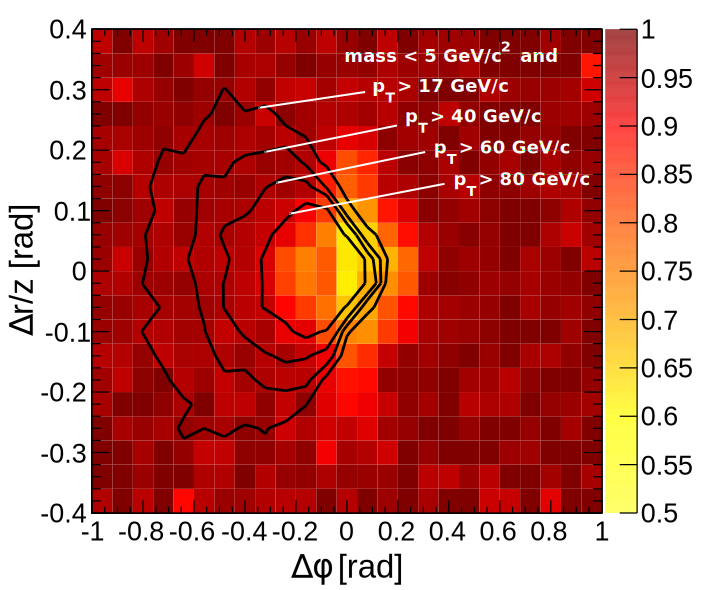
\includegraphics[width=0.48\linewidth]{PLOTS/endcap_dphidr_HLTMu11_09_21.pdf} \hfill
\includegraphics[width=0.48\linewidth]{PLOTS/trigger_turnonMu11.pdf}

\caption{Diagnostic of HLT\_Mu11 $p_T$ dependence in $0.9 < |\eta| <
  2.1$.  Left: trigger efficiency (color scale) with one $p_T >
  12$~GeV/$c$ muon, the other unconstrained, as a function of
  separation of muons in the muon system.  Different mass/momentum
  combinations (the labeled contour lines) sample this spot to
  differing degrees.  The trigger turn-on curve in the spot is
  unaffected; it is the plateau efficiency that is
  lowered. \label{fig:triggersimulation2}}
\end{figure}

%% To check the trigger efficiency with data, we use a standard
%% tag-and-probe technique, adapted for our analysis.  Selecting $J/\psi
%% \to \mu\mu$ events reconstructed offline with $3.0 < \mbox{dimuon
%%   mass} < 3.2$~GeV/$c^2$, we require one daughter to have $p_T >
%% 12$~GeV/$c$, $|\eta| < 0.9$ and to be matched to an HLT\_Mu11 trigger
%% object.  We additionally put a requirement on $\Delta \phi =
%% \phi_{\mu^+} - \phi_{\mu^-}$ for muon trajectories propagated to a
%% cylinder of radius 600~cm, centered on the beamline (barrel
%% station~3).  We allow only $\Delta \phi < -0.3$ to exclude cases in
%% which StandAloneMuon reconstruction of one muon (part of the HLT
%% trigger algorithm) would interfere with the StandAloneMuon
%% reconstruction of the other, implicitly biasing the efficiency
%% measurement (see Fig.~\ref{fig:triggerstudybias}).

%% \begin{figure}
%% \begin{center}
%% \includegraphics[width=0.48\linewidth]{PLOTS/barrel_dphi_bypt_StandAloneMuon_09.pdf} \hfill
%% \includegraphics[width=0.48\linewidth]{PLOTS/barrel_dphidr_StandAloneMuon.pdf}
%% \end{center}

%% \caption{Probability of reconstructing two StandAloneMuons as a
%%   function of muon trajectories propagated to the muon barrel (at
%%   least one $p_T > 12$~GeV/$c$ muon, and both muons have $|\eta| <
%%   0.9$).  The StandAloneMuon inefficiency is asymmetric because of
%%   muon energy loss in material between the origin and the muon system
%%   ($\Delta \phi$ is defined such that lost energy yields positive
%%   $\Delta \phi$), and is double-peaked from the two oppositely-charged
%%   track helix topologies (``seagulls'' and ``cowboys'').  To avoid
%%   interference between the tag and the probe in the data-driven
%%   efficiency measurement, we require $\Delta \phi <
%%   -0.3$. \label{fig:triggerstudybias}}
%% \end{figure}

%% The data-driven trigger efficiency is defined as the fraction of
%% events from the sample above in which the second muon is also matched
%% to an HLT\_Mu11 trigger object.







\appendix

\section{Motivation for trigger choice}
\label{sec:motivation_for_trigger_choice}

\end{document}


%% \pagebreak

%% CMS muon triggers are efficient for nearby muons within certain
%% boundaries that motivate our choice of the unisolated, single-muon
%% trigger and the offline acceptance cuts to guarantee uniform
%% efficiency afte cuts.  The boundaries are:
%% \begin{itemize}
%% \item $p_T$ (the threshold curves) and $|\eta|$ (extent of the
%%   detector), well-documented elsewhere (\fixme{reference?});
%% \item double-muon triggers (e.g.\ HLT\_DoubleMu3) are inefficient when
%%   the muons cross in the muon system (moderate boost, depends on
%%   kinematics);
%% \item track-based isolation (e.g.\ in HLT\_IsoMu9) excludes muons that
%%   are too close to one another in the pixel detector (very high boost
%%   only);
%% \item the L1 endcap trigger is inefficient when the muons cross in the
%%   muon system.  (\fixme{Only known to be due to L1 by process of
%%     elimination and one brief test, not a complete study that
%%     identifies the underlying cause.})
%% \end{itemize}
%% The last condition motivates the acceptance requirement of one
%% high-momentum muon in the barrel ($|\eta| < 1$).

%% To investigate trigger and offline reconstruction efficiencies, a
%% special Monte Carlo was generated with dimuons uniformly distributed
%% in mass (a random mass was chosen in each event), pair $p_T$, and pair
%% $\eta$.  Instead of realistically modeling any physical process, this
%% ``dimuon gun'' covers the space of possible dimuons in a physically
%% reasonable way, allowing us to search for inefficient regions.  All
%% trigger efficiencies quoted below are efficiencies for L1 and HLT
%% combined, labeled by HLT path name.

%% The HLT\_DoubleMu3 trigger has a complex efficiency profile for
%% dimuons, presented in Fig.~\ref{fig:doublemu_trigger} with offline
%% StandAloneMuon reconstruction efficiency for comparison.  The
%% HLT\_DoubleMu3 trigger requires two GlobalMuons to be reconstructed in
%% the HLT, and thus implicitly requires two StandAloneMuons.  The
%% StandAloneMuon profile reproduces the inefficiency between barrel
%% wheels of HLT\_DoubleMu3, but not the inefficiency at high $|\eta|$.
%% Both inefficiency patterns are only substantial for low-mass,
%% high-momentum dimuons: muons that are nearly parallel and overlapping
%% in the muon system.

%% \begin{figure}
%% \includegraphics[width=0.45\linewidth]{PLOTS/masseta_DMu3.pdf} \hfill
%% \includegraphics[width=0.45\linewidth]{PLOTS/pteta_mass5cut_DMu3.pdf}

%% \includegraphics[width=0.45\linewidth]{PLOTS/masseta_StandAloneMuon.pdf} \hfill
%% \includegraphics[width=0.45\linewidth]{PLOTS/pteta_mass5cut_StandAloneMuon.pdf}

%% \caption{Top two plots: efficiency (color scale) of HLT\_DoubleMu3
%%   trigger as a function of dimuon mass, $\eta$, and $p_T$.  Bottom two
%%   plots: probability to reconstruct two StandAloneMuons, a
%%   prerequisite for the HLT\_DoubleMu3 trigger.  Plots on the right are
%%   for mass $<$ 5~GeV/$c^2$ only. \label{fig:doublemu_trigger}}
%% \end{figure}

%% The effect of isolation in HLT\_IsoMu9 is shown in
%% Fig.~\ref{fig:isolation_trigger} by comparison with HLT\_Mu9.  Both
%% exhibit the same inefficiency at high $|\eta|$, but HLT\_IsoMu9
%% additionally has an inefficiency for $p_T \gtrsim 50$~GeV/$c$ dimuons
%% at $|\eta| < 0.5$.  The isolation is implemented by requiring an
%% absence of pixel-tracks near the triggered muon, which is violated in
%% high-momentum dimuons.

%% \begin{figure}
%% \includegraphics[width=0.45\linewidth]{PLOTS/masseta_pluscut_IsoMu9.pdf} \hfill
%% \includegraphics[width=0.45\linewidth]{PLOTS/pteta_mass5cut_pluscut_IsoMu9.pdf}

%% \includegraphics[width=0.45\linewidth]{PLOTS/masseta_pluscut_Mu9.pdf} \hfill
%% \includegraphics[width=0.45\linewidth]{PLOTS/pteta_mass5cut_pluscut_Mu9.pdf}

%% \caption{Top two plots: efficiency (color scale) of HLT\_IsoMu9
%%   trigger as a function of dimuon mass, $\eta$, and $p_T$.  Bottom two
%%   plots: efficiency of HLT\_Mu9, the same trigger without isolation.
%%   The denominator for all efficiencies includes at least one $p_T >
%%   15$~GeV/$c$ muon, and mass $<$ 5~GeV/$c^2$ for plots on the
%%   right. \label{fig:isolation_trigger}}
%% \end{figure}

%% Figure~\ref{fig:efficiency_vs_eta} shows HLT\_IsoMu9, HLT\_Mu9, and
%% HLT\_Mu11 versus $\eta$ only, so that quantitative efficiencies can be
%% read from the plot.  The unisolated, single-muon triggers have
%% 95--100\% efficiency in the barrel region ($|\eta| < 1$) but the
%% efficiency curves to zero in the endcap, independent of $p_T$.

%% \begin{figure}
%% \includegraphics[width=0.32\linewidth]{PLOTS/eta_mass5cut_pluscut_IsoMu9.pdf} \hfill
%% \includegraphics[width=0.32\linewidth]{PLOTS/eta_mass5cut_pluscut_Mu9.pdf} \hfill
%% \includegraphics[width=0.32\linewidth]{PLOTS/eta_mass5cut_pluscut_Mu11.pdf}

%% \caption{Trigger efficiency for HLT\_IsoMu9 (left), HLT\_Mu9 (middle),
%%   and HLT\_Mu11 (right) for muon pairs in which both muons are in the
%%   specified $p_T$ ranges.  All muon pairs in this sample have
%%   invariant mass $<$ 5~GeV/$c^2$ and at least one $p_T > 15$~GeV/$c$
%%   muon. \label{fig:efficiency_vs_eta}}
%% \end{figure}

%% This inefficiency is strongest for muons that cross each other in the
%% muon endcap.  This can be seen by plotting the efficiency as a
%% function of difference in muon trajectories evaluated in the detector,
%% rather than the interaction point.  Two planes, one at 700~cm and the
%% other at $-$700~cm from the interaction point were used to represent
%% the two endcaps, and generator-level muon trajectories were propagated
%% through the CMS magnetic field to these planes, where their positions
%% were compared in two dimensions: $\Delta \phi$ (difference in
%% azimuthal angle) and $\Delta r/z$ (difference in radial position
%% divided by 700~cm).

%% Figure~\ref{fig:endcap_trigger_spot} shows the HLT\_Mu11 endcap
%% efficiency as a function of crossing distance and $p_T$: the
%% efficiency is localized to muons that nearly cross one another, but is
%% independent of $p_T$.  The probability to reconstruct one of the two
%% muons as an offline StandAloneMuon or GlobalMuon is nearly 100\% for
%% all crossing distances, $p_T$, and $\eta$, implying that this
%% inefficiency is in L1, rather than HLT.  \fixme{I have one plot from
%%   Vadim by e-mail showing positively that this is an L1 issue (rather
%%   than just deducing it from process of elimination, as I do here, but
%%   it's a single plot versus $\Delta R$.  It would be good to put it in
%%   the same form as the rest of these, possibly investigating it with
%%   more variables ($\Delta \phi$, $\Delta r/z$, $p_T$, $\eta$).}

%% \begin{figure}
%% \includegraphics[width=0.45\linewidth]{PLOTS/endcap_dphidr_HLTMu11.pdf} \hfill
%% \includegraphics[width=0.45\linewidth]{PLOTS/trigger_turnonMu11.pdf}

%% \caption{Left: endcap ($|\eta| < 1$) HLT\_Mu11 efficiency as a
%%   function of where muon trajectories cross one another in the endcap
%%   (a plane at $\pm$700~cm).  Right: HLT\_Mu11 efficiency ($1 < |\eta|
%%   < 2.1$) as a function of the positive-muon $p_T$ (the negative muon
%%   has $p_T < 9$~GeV/$c$ to avoid satisfying the trigger).  The
%%   ``spot'' is defined as $|\Delta \phi| < 0.2$ and $|\Delta r/z| <
%%   0.1$. \label{fig:endcap_trigger_spot}}
%% \end{figure}

%% If we did not explicitly require one offline high-$p_T$ muon with
%% $|\eta| < 1$, then different physics models would be sensitive to this
%% inefficiency to different degrees, depending on how they populate the
%% $p_T$, $\eta$ plane and what masses they predict.  It would be
%% difficult to provide this information in a useful way, since it
%% depends on several variables, some of which are obtained by
%% propagating muon trajectories through the CMS magnetic field.  We
%% therefore require at least one offline muon with $p_T > 15$~GeV/$c$,
%% $|\eta| < 1$ muon in every signal channel, thus guaranteeing that
%% HLT\_Mu9 and HLT\_Mu11 are in the plateau region of $p_T$ and are
%% insensitive to whether muons cross in the detector.

%% Measurement of the trigger efficiency in the plateau region is covered
%% in Sec.~\ref{sec:measuring_efficiencies}.

%% \section{Offline muon reconstruction and identification}

%% All offline muons in this analysis are selected to have the following
%% properties:
%% \begin{itemize}
%% \item $p_T > 5$~GeV/$c$ and $|\eta| < 2.4$;
%% \item identified with the TrackerMuon algorithm (tracker-track
%%   matched to muon segments, the inside-out muon identification);
%% \item at least two fully arbitrated (SegmentAndTrackArbitration) muon
%%   segments;
%% \item number of hits in the tracker $\ge$ 8;
%% \item track $\chi^2/N_\s{dof}$ in the tracker $<$ 4.
%% \end{itemize}

%% \subsection{Offline muon efficiency}
%% \label{sec:offline_muon_efficiency}

%% The most unusual choice in the above is the use of TrackerMuons for
%% high-momentum muons: this is motivated by the fact that the
%% TrackerMuon (inside-out) algorithm is more robust than the GlobalMuon
%% (outside-in) algorithm for identifying all muons when they cross one
%% another in the muon system.  The point of failure for the GlobalMuon
%% algorithm is in the stage where a StandAloneMuon is built from
%% segments.  The TrackerMuon algorithm only requires segments, so it is
%% insensitive to this effect.

%% To quantify this inefficiency, we again cover all possible dimuon
%% kinematics with a dimuon gun Monte Carlo and we propagate generator-level muon
%% trajectories through the CMS magnetic field to the muon system, then
%% plot efficiency as a function of the distance between the muons.  Both
%% of these techniques were used in
%% Sec.~\ref{sec:region_of_constant_trigger_efficiency}, but here we plot
%% the probability of reconstructing {\it both} muons offline, rather than the
%% probability of triggering on one of the two.  For barrel muons
%% ($|\eta| < 1$), this surface is a cylinder centered on the beamline
%% with radius 600~cm.  For endcap muons ($|\eta| > 1$), this surface is
%% a plane at 700~cm or $-$700~cm from the interaction point,
%% perpendicular to the beamline (see Fig.~\ref{fig:cms_quarterview}).
%% The distance of separation is quantified in the barrel as $\Delta
%% \phi$ (difference in azimuthal angles) and $\Delta z/r$ (displacement
%% parallel with the beamline divided by 600~cm), and in the endcap, the
%% distance of separation is $\Delta \phi$ and $\Delta r/z$ (radial
%% displacement toward or away from the beamline divided by 700~cm).
%% Reconstruction probabilities are shown in Fig.~\ref{fig:barrel_dphidr}
%% for the barrel and Fig.~\ref{fig:endcap_dphidz} for the endcap.

%% \begin{figure}
%% \begin{center}
%% 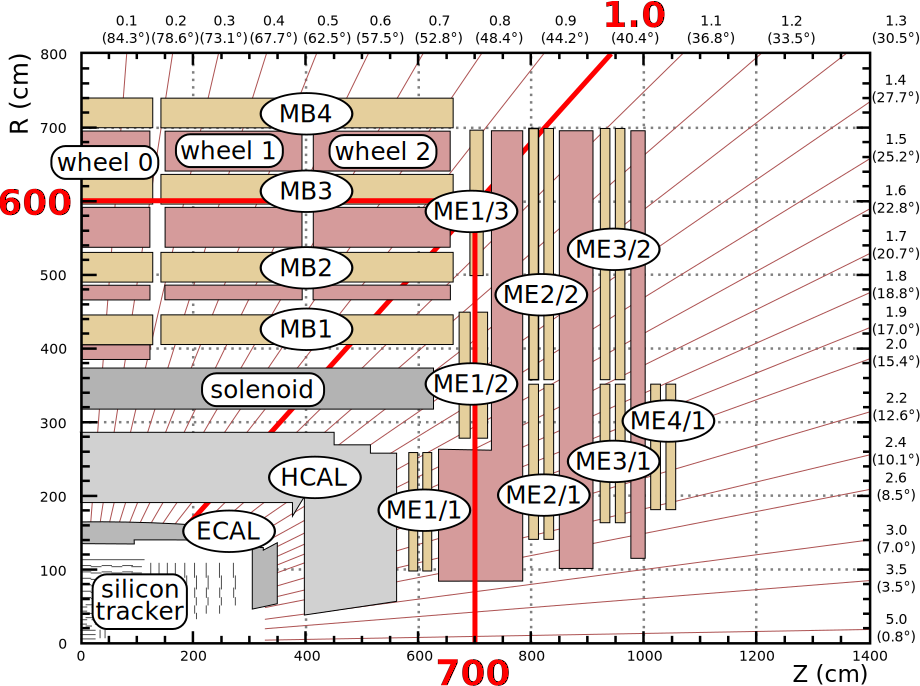
\includegraphics[width=0.6\linewidth]{PLOTS/cms_quarterview.pdf}
%% \end{center}

%% \caption{CMS quarter-view illustrating the cylindrical surface with
%%   600~cm radius (barrel, $|\eta| < 1$) and plane 700~cm from the
%%   beamspot (endcap, $1 < |\eta| < 2.4$) used to quantify
%%   reconstruction efficiency as a function of crossing distance in the
%%   muon system. \label{fig:cms_quarterview}}
%% \end{figure}

%% \begin{figure}
%% \includegraphics[width=0.32\linewidth]{PLOTS/barrel_dphidr_StandAloneMuon.pdf} \hfill
%% \includegraphics[width=0.32\linewidth]{PLOTS/barrel_dphidr_GlobalMuon.pdf} \hfill
%% \includegraphics[width=0.32\linewidth]{PLOTS/barrel_dphidr_TrackerMuon.pdf}

%% \includegraphics[width=0.32\linewidth]{PLOTS/barrel_dphi_bypt_StandAloneMuon.pdf} \hfill
%% \includegraphics[width=0.32\linewidth]{PLOTS/barrel_dphi_bypt_GlobalMuon.pdf} \hfill
%% \includegraphics[width=0.32\linewidth]{PLOTS/barrel_dphi_bypt_TrackerMuon.pdf}

%% \caption{Probability of reconstructing two muons (both $|\eta| < 1$)
%%   as StandAloneMuons (left), GlobalMuons (middle), and TrackerMuons
%%   with quality cuts (right).  Top row: efficiency versus distance
%%   between the muon trajectories on a cylinder of radius 600~cm.
%%   Bottom row: profile in $\Delta \phi$ ($|\Delta z/r| < 0.3$) with
%%   both muons in a given $p_T$ range.  \label{fig:barrel_dphidr}}
%% \end{figure}

%% \begin{figure}
%% \includegraphics[width=0.32\linewidth]{PLOTS/endcap_dphidr_StandAloneMuon.pdf} \hfill
%% \includegraphics[width=0.32\linewidth]{PLOTS/endcap_dphidr_GlobalMuon.pdf} \hfill
%% \includegraphics[width=0.32\linewidth]{PLOTS/endcap_dphidr_TrackerMuon.pdf}

%% \includegraphics[width=0.32\linewidth]{PLOTS/endcap_dphi_bypt_StandAloneMuon.pdf} \hfill
%% \includegraphics[width=0.32\linewidth]{PLOTS/endcap_dphi_bypt_GlobalMuon.pdf} \hfill
%% \includegraphics[width=0.32\linewidth]{PLOTS/endcap_dphi_bypt_TrackerMuon.pdf}

%% \caption{Probability of reconstructing two muons (both $|\eta| < 1$)
%%   as StandAloneMuons (left), GlobalMuons (middle), and TrackerMuons
%%   with quality cuts (right).  Top row: efficiency versus distance
%%   between the muon trajectories on a plane $\pm$700~cm from the
%%   interaction point.  Bottom row: profile in $\Delta \phi$ ($|\Delta
%%   r/z| < 0.1$) with both muons in a given $p_T$
%%   range.  \label{fig:endcap_dphidz}}
%% \end{figure}

%% In all cases, the GlobalMuon efficiency follows the StandAloneMuon
%% efficiency, and the reconstruction efficiency of two TrackerMuons is
%% nearly independent of crossing distance.  (The arbitration requirement
%% introduces a 5\% drop in efficiency for $|\Delta \phi| < 0.1$ muons in
%% the endcap.)  The barrel profile is complicated by the fact that
%% propagated generator-level muons don't accurately predict the position
%% of a real muon in the barrel, since real muons can scatter or lose
%% energy to a final-state photon.  This is why the efficiency curve is
%% smeared toward positive $\Delta \phi$ (energy loss in either muon
%% would result in positive $\Delta \phi$) for low-momentum muons, forms
%% two inefficient regions for mid-range momenta (two helix topologies,
%% often called ``cowboys'' and ``seagulls''), and a single inefficient
%% region for $\Delta \phi = 0$.

%% To avoid these reconstruction inefficiencies, we use TrackerMuons for
%% all offline muon identification.
%% Section~\ref{sec:measuring_efficiencies} describes how this efficiency
%% is actually measured and applied per muon.

%% \subsection{Offline muon fake rate}

%% Raw TrackerMuons only require a tracker-track to be consistent with a
%% segment in the muon system, but in dense tracking environments,
%% several tracks from hadronic particles may point to the segments of a
%% real muon and become incorrectly identified as additional muons.  This
%% would lead to an unacceptably high muon fake rate.  GlobalMuons, on
%% the other hand, are known to have low fake rates, but with the
%% inefficiency for nearby muons described in
%% Sec.~\ref{sec:offline_muon_efficiency}.

%% TrackerMuons can be selected with the same purity as GlobalMuons by
%% requiring at least two fully arbitrated segments.  Full arbitration
%% (SegmentAndTrackArbitration) requires only one segment to match to
%% each tracker-track per chamber (SegmentArbitration) and only one
%% tracker-track to match to each segment (TrackArbitration).  The actual
%% cut is placed on the number of matched segments with this property.
%% This emulates an implicit condition in GlobalMuon reconstruction:
%% segments used to build one muon are not available for any other muons.

%% Using a sample of realistic background Monte Carlo (inclusive muons
%% with $\hat{p}_T > 30$~GeV/$c$) in
%% Fig.~\ref{fig:tracks_lastpage_allreal}, we show the distribution of
%% the number of tracks for raw TrackerMuons, TrackerMuons with at least
%% two segments and at least two arbitrated segments, and GlobalMuons as
%% a reference.  In Fig.~\ref{fig:tracks_lastpage}, we show this plot for
%% different numbers of matched generator-level muons.  Both the number
%% of reconstructed GlobalMuons and fully arbitrated TrackerMuons peak at
%% the true number of muons with similar tails, demonstrating a similar
%% fake rate.

%% \begin{figure}
%% \begin{center}
%% \includegraphics[height=0.6\linewidth, angle=90]{PLOTS/tracks_lastpage_allreal.pdf}
%% \end{center}

%% \caption{Number of reconstructed muons in an inclusive muon
%%   backgrounds sample with $\hat{p}_T > 30$~GeV/$c$.  The fully arbitrated
%%   TrackerMuons has a purity similar to
%%   GlobalMuons. \label{fig:tracks_lastpage_allreal}}
%% \end{figure}

%% \begin{figure}
%% \begin{center}
%% \includegraphics[height=0.45\linewidth, angle=90]{PLOTS/tracks_lastpage_0real.pdf} \hfill
%% \includegraphics[height=0.45\linewidth, angle=90]{PLOTS/tracks_lastpage_1real.pdf}

%% \includegraphics[height=0.45\linewidth, angle=90]{PLOTS/tracks_lastpage_2real.pdf} \hfill
%% \includegraphics[height=0.45\linewidth, angle=90]{PLOTS/tracks_lastpage_3real.pdf}

%% \includegraphics[height=0.45\linewidth, angle=90]{PLOTS/tracks_lastpage_4real.pdf} \hfill
%% \includegraphics[height=0.45\linewidth, angle=90]{PLOTS/tracks_lastpage_5real.pdf}
%% \end{center}

%% \caption{Number of reconstructed muons as in
%%   Fig.~\ref{fig:tracks_lastpage_allreal}, split by the number of true
%%   muons in the event (unique MC matches).  In each case, the fully
%%   arbitrated TrackerMuons and the GlobalMuons peak at the true number
%%   of muons with similar tails. \label{fig:tracks_lastpage}}
%% \end{figure}

%% The number of tracker hits and tracker-track $\chi^2$ cuts have
%% negligible impact on efficiency and fake rates, but they are standard
%% track quality cuts.

%% \section{Measuring trigger and offline muon efficiencies}
%% \label{sec:measuring_efficiencies}

%% \fixme{Need to get this number from somewhere.  Surely it should be
%%   $J/\psi \to \mu\mu$ tag-and-probe, but with our cuts to be
%%   completely in the plateau efficiency region.  It should be one
%%   event-level correction for the trigger efficiency and one efficiency
%%   factor per muon for the offline reconstruction.}

%% \subsection{Mu-jet clustering and fundamental dimuon decomposition}

%% Complicated lepton-jets cascades can make it difficult to identify
%% which muons belong to which resonance, and therefore possibly
%% misreconstruct the masses and fail to identify the signature.  To be
%% prepared for any high-multiplicity muon event with many boosted
%% resonances, it is necessary to have a procedure to organize the muons
%% into likely pairings and groups.  Our organizational procedure has two
%% steps: (1) groups of ``close-by'' muons are grouped into mu-jets with
%% arbitrarily many mu-jets per group, and (2) mu-jets are analyzed for
%% the most likely decomposition into fundamental dimuons belonging to the
%% lowest-mass state in the hidden spectrum.

%% To cluster muons into mu-jets, we identify opposite-sign pairs of
%% close-by muons according to pairwise invarant mass ($m_\s{inv}$) and
%% pairwise vertex compatibility ($P_\s{vertex}$) and group all close-by
%% muons.  Muon tracks with very small angular separation ($\Delta R <
%% 0.01$) have an increased probability of failing the vertex fit
%% (Fig.~\ref{fig:vertex_probability_dip}), so we define two
%% oppositely-charged muons as being close-by if the following is
%% satisfied:
%% \begin{equation}
%% \left( m_\s{inv} < 5\mbox{ GeV/$c^2$ {\bf and} }P_\s{vertex} >
%% 0.01\right)\mbox{ {\bf or} }\Delta R < 0.01.
%% \label{eqn:closeness}
%% \end{equation}
%% This definition has the following consequences:
%% \begin{itemize}
%% \item any resonance with mass $<$ 5~GeV/$c^2$ decaying into two properly
%%   reconstructed muons is guaranteed to be considered close-by with
%%   99\% probability, regardless of momentum;
%% \item muons originating from two different points in space are
%%   suppressed ($b \to \mu \mu X$ has about 75\% efficiency);
%% \item very small angle dimuons are not lost due to failure of the
%%   vertex fitter, but only these dimuons, with a relativistic boost of
%%   $\gamma > 100$, are exempt from the vertex test.
%% \end{itemize}

%% \begin{figure}
%% \begin{center}
%% 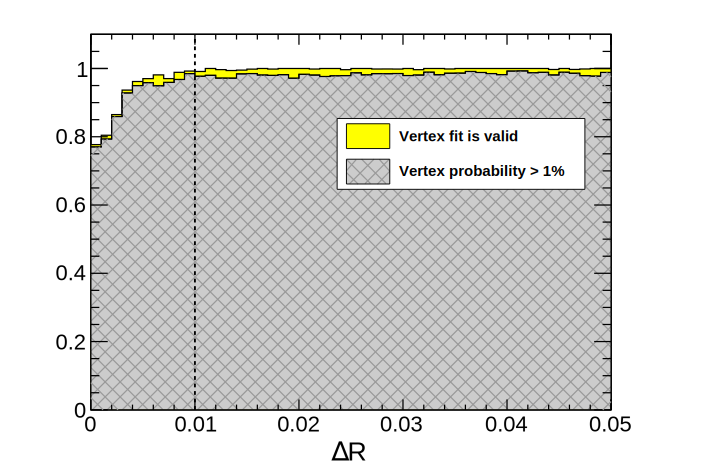
\includegraphics[width=0.6\linewidth]{PLOTS/vertex_probability_dip.pdf}
%% \end{center}

%% \caption{Probability of vertex fit failure and vertex compatibility
%%   $>$ 1\% as a function of geometric separation ($\Delta R =
%%   \sqrt{(\Delta \phi)^2 + (\Delta
%%     \eta)^2}$). \label{fig:vertex_probability_dip}}
%% \end{figure}

%% Close-by pairs are iteratively grouped into mu-jets until every pair
%% of close-by muons are in the same mu-jet.  Closeness is always defined
%% between muons, never an averaged group of muons, so the clustering
%% procedure is independent of the order in which it is applied.  Whole
%% decay chains in which the most massive state in the cascade has a mass
%% under 5~GeV/$c^2$ would also be grouped into a single mu-jet, assuming
%% that all final state muons are reconstructed.

%% To search for a mass peak corresponding to the lightest state in the
%% hidden sector, mu-jets are decomposed into fundamental dimuons.  In a
%% mu-jet with many muons, there can be several ways to partition the
%% muons into oppositely-signed pairs.  One of these combinations
%% minimizes the quantity
%% \begin{equation}
%% \chi^2_{\Delta m} = \sum_i^\s{OS pairs} \, \sum_{j > i}^\s{OS pairs}
%% \left(m_i - m_j\right)^2.
%% \end{equation}
%% This set of masses is most consistent with multiple instances of $m_1
%% \to \mu\mu$ overlapping one another in the same event.

%% Figures~\ref{fig:eff_mujetform}--\ref{fig:eff_trigger_inplateau}
%% demonstrate the uniformity of mu-jet efficiency over masses of
%% $2m_\mu$--5~GeV/$c^2$ and momenta up to 100~GeV/$c$.
%% Figure~\ref{fig:eff_mujetform} shows the algorithmic efficiency,
%% determined primarily by the $P_\s{vertex} > 1$\% constraint.
%% Figure~\ref{fig:eff_mujetreco} is the combined probability of track
%% reconstruction and the clustering algorithm.  The same for events with
%% one $p_T > 15$~GeV/$c$, $|\eta| < 1$ muon (to satisfy the trigger) is
%% shown in Fig.~\ref{fig:eff_mujetreco_inplateau}: it essentially raises
%% the minimum mu-jet $p_T$ from 10~GeV/$c$ to 20~GeV/$c$.  Finally,
%% Fig.~\ref{fig:eff_trigger_inplateau} shows the efficiency of the
%% trigger, reconstruction, and mu-jet clustering.

%% \begin{figure}
%% \includegraphics[width=0.24\linewidth]{PLOTS/eff_mujetform_masspt.pdf} \hfill
%% \includegraphics[width=0.24\linewidth]{PLOTS/eff_mujetform_massonly.pdf} \hfill
%% \includegraphics[width=0.24\linewidth]{PLOTS/eff_mujetform_ptonly.pdf} \hfill
%% \includegraphics[width=0.24\linewidth]{PLOTS/eff_mujetform_eta.pdf}

%% \caption{Probability to form a mu-jet, given two reconstructed
%%   muons. \label{fig:eff_mujetform}}
%% \end{figure}

%% \begin{figure}
%% \includegraphics[width=0.24\linewidth]{PLOTS/eff_mujetreco_masspt.pdf} \hfill
%% \includegraphics[width=0.24\linewidth]{PLOTS/eff_mujetreco_massonly.pdf} \hfill
%% \includegraphics[width=0.24\linewidth]{PLOTS/eff_mujetreco_ptonly.pdf} \hfill
%% \includegraphics[width=0.24\linewidth]{PLOTS/eff_mujetreco_eta.pdf}

%% \caption{Probability to reconstruct two muons and form a mu-jet, given
%%   two muons with $p_T > 5$~GeV/$c$ and $|\eta| < 2.4$. \label{fig:eff_mujetreco}}
%% \end{figure}

%% \begin{figure}
%% \includegraphics[width=0.24\linewidth]{PLOTS/eff_mujetreco_inplateau_masspt.pdf} \hfill
%% \includegraphics[width=0.24\linewidth]{PLOTS/eff_mujetreco_inplateau_massonly.pdf} \hfill
%% \includegraphics[width=0.24\linewidth]{PLOTS/eff_mujetreco_inplateau_ptonly.pdf} \hfill
%% \includegraphics[width=0.24\linewidth]{PLOTS/eff_mujetreco_inplateau_eta.pdf}

%% \caption{Probability to reconstruct two muons and form a mu-jet, given
%%   two muons, one with $p_T > 12$~GeV/$c$ and $|\eta| < 1$, the other
%%   with $p_T > 5$~GeV/$c$ and $|\eta| < 2.4$.  \label{fig:eff_mujetreco_inplateau}}
%% \end{figure}

%% \begin{figure}
%% \includegraphics[width=0.24\linewidth]{PLOTS/eff_trigger_inplateau_masspt.pdf} \hfill
%% \includegraphics[width=0.24\linewidth]{PLOTS/eff_trigger_inplateau_massonly.pdf} \hfill
%% \includegraphics[width=0.24\linewidth]{PLOTS/eff_trigger_inplateau_ptonly.pdf} \hfill
%% \includegraphics[width=0.24\linewidth]{PLOTS/eff_trigger_inplateau_eta.pdf}

%% \caption{Probability to trigger, reconstruct, and form a mu-jet, given
%%   two muons, one with $p_T > 12$~GeV/$c$ and $|\eta| < 1$, the other
%%   with $p_T > 5$~GeV/$c$ and $|\eta| < 2.4$. \label{fig:eff_trigger_inplateau}}
%% \end{figure}

%% \subsection{Mu-jet isolation}

%% Although isolation is not applied to any signal regions, it is a
%% useful tool for identifying background sources in the control samples
%% and would be used to study a signal if one is discovered.  Standard
%% muon isolation is inappropriate because nearby muons would fall within
%% each other's isolation cones.  We therefore define a new track-based
%% isolation variable that excludes all muons from the set of tracks.
%% The isolation $Iso$ of a mu-jet is
%% \begin{equation}
%% Iso(R^\s{max}, p_T^\s{min}) = \sum_\s{non-$\mu$ tracks} \left\{ \begin{array}{c l} p_T &
%%   \mbox{ if $\Delta R < R^\s{max}$ and $p_T > p_T^\s{min}$} \\ 0 &
%%   \mbox{ otherwise} \end{array} \right.
%% \label{eqn:isolation}
%% \end{equation}
%% where $\Delta R$ is $\sqrt{(\Delta \phi)^2 + (\Delta \eta)^2}$ with
%% respect to the mu-jet's momentum axis (vector sum of all grouped muon
%% momenta).  The cone radius $\Delta R < R^\s{max}$ and track momentum
%% threshold $p_T^\s{min}$ are optimized such that Standard Model
%% backgrounds from $b$-jets are roughly uniform in the range $0 < Iso
%% \lesssim 10$~GeV/$c$.

%% Distributions of $Iso(R^\s{max}, p_T^\s{min})$ in Monte Carlo samples
%% covering the range of backgrounds for our signal topologies are
%% presented in Figs.~\ref{fig:inclusiveMu_iso} (inclusive muon with
%% $\hat{p}_T > 30$~GeV/$c$), \ref{fig:inclusiveMuPt100_iso} (inclusive
%% muon with $\hat{p}_T > 100$~GeV/$c$) and \ref{fig:inclBB4mu_iso}
%% ($b\bar{b} \to 4\mu \, X$ in two mu-jets).  All have a roughly flat
%% region in $0 < Iso < 9$~GeV/$c$ for $\Delta R < R^\s{max} =
%% 0.4$ and $p_T^\s{min} = 1.5$~GeV/$c$ (lower-left plot, dotted blue
%% curve in all Figures).

%% \begin{figure}
%% \mbox{ } \hfill \includegraphics[width=0.4\linewidth]{PLOTS/inclusiveMu_iso02.pdf} \hfill
%% \includegraphics[width=0.4\linewidth]{PLOTS/inclusiveMu_iso03.pdf} \hfill \mbox{ }

%% \mbox{ } \hfill \includegraphics[width=0.4\linewidth]{PLOTS/inclusiveMu_iso04.pdf} \hfill
%% \includegraphics[width=0.4\linewidth]{PLOTS/inclusiveMu_iso05.pdf} \hfill \mbox{ }

%% \caption{Inclusive muon MC ($\hat{p}_T > 30$~GeV/$c$) distributions of
%%   $Iso(R^\s{max}, p_T^\s{min})$.  Histogram bins have the same width
%%   as the $p_T^\s{min}$ threshold. \label{fig:inclusiveMu_iso}}
%% \end{figure}

%% \begin{figure}
%% \mbox{ } \hfill \includegraphics[width=0.4\linewidth]{PLOTS/inclusiveMuPt100_iso02.pdf} \hfill
%% \includegraphics[width=0.4\linewidth]{PLOTS/inclusiveMuPt100_iso03.pdf} \hfill \mbox{ }

%% \mbox{ } \hfill \includegraphics[width=0.4\linewidth]{PLOTS/inclusiveMuPt100_iso04.pdf} \hfill
%% \includegraphics[width=0.4\linewidth]{PLOTS/inclusiveMuPt100_iso05.pdf} \hfill \mbox{ }

%% \caption{Inclusive muon MC ($\hat{p}_T > 100$~GeV/$c$) distributions of
%%   $Iso(R^\s{max}, p_T^\s{min})$.  Histogram bins have the same width
%%   as the $p_T^\s{min}$ threshold. \label{fig:inclusiveMuPt100_iso}}
%% \end{figure}

%% \begin{figure}
%% \mbox{ } \hfill \includegraphics[width=0.4\linewidth]{PLOTS/inclBB4mu_iso02.pdf} \hfill
%% \includegraphics[width=0.4\linewidth]{PLOTS/inclBB4mu_iso03.pdf} \hfill \mbox{ }

%% \mbox{ } \hfill \includegraphics[width=0.4\linewidth]{PLOTS/inclBB4mu_iso04.pdf} \hfill
%% \includegraphics[width=0.4\linewidth]{PLOTS/inclBB4mu_iso05.pdf} \hfill \mbox{ }

%% \caption{Muon-enriched $b\bar{b} \to 4\mu \, X$ MC ($\hat{p}_T >
%%   30$~GeV/$c$) distributions of $Iso(R^\s{max}, p_T^\s{min})$.
%%   Histogram bins have the same width as the $p_T^\s{min}$
%%   threshold. \label{fig:inclBB4mu_iso}}
%% \end{figure}

%% Figure~\ref{fig:highpileup_iso} shows the same distributions for an
%% idealized signal: a muon pair-gun with high pile-up (average of 5
%% interactions per crossing).  From this we see that the isolation does
%% not veto real muon pairs (most of which are within $\Delta R < 0.4$)
%% and is insensitive to pile-up.  In realistic lepton jets scenarios,
%% mu-jets may be produced with $e^+e^-$ or $\pi\pi$ and fail isolation
%% for a fraction of the events (large for $Z$-like couplings, small for
%% Higgs-like couplings).

%% \begin{figure}
%% \mbox{ } \hfill \includegraphics[width=0.4\linewidth]{PLOTS/highpileup_iso02.pdf} \hfill
%% \includegraphics[width=0.4\linewidth]{PLOTS/highpileup_iso03.pdf} \hfill \mbox{ }

%% \mbox{ } \hfill \includegraphics[width=0.4\linewidth]{PLOTS/highpileup_iso04.pdf} \hfill
%% \includegraphics[width=0.4\linewidth]{PLOTS/highpileup_iso05.pdf} \hfill \mbox{ }

%% \caption{Muon pair-gun MC with high pile-up (average of 5 interactions
%%   per crossing) distributions of $Iso(R^\s{max}, p_T^\s{min})$.
%%   Histogram bins have the same width as the $p_T^\s{min}$
%%   threshold. \label{fig:highpileup_iso}}
%% \end{figure}

%% The mu-jet clustering is defined with a cut on pairwise invariant
%% mass, while isolation is defined with a geometric cone.  It is
%% therefore possible for two distinct mu-jets to have overlapping
%% isolation cones.  In such a case, the values of the isolation
%% variables of the two mu-jets would be correlated by sharing tracks.
%% However, the main source of backgrounds to two mu-jet events,
%% $b\bar{b} \to 2\mu, \, 2\mu$, are overwhelmingly back-to-back in
%% $\phi$.  Figure~\ref{fig:inclBB4mu_is_usually_backtoback} shows the
%% separation of pairs of mu-jets from $b\bar{b}$: only very boosted
%% $b\bar{b}$ systems produce mu-jets with overlapping isolation cones
%% ($\Delta R \le 2R^\s{max} = 0.8$).

%% \begin{figure}
%% \begin{center}
%% \includegraphics[width=0.6\linewidth]{PLOTS/inclBB4mu_is_usually_backtoback.pdf}
%% \end{center}

%% \caption{Separation of mu-jets in $b\bar{b} \to 2\mu, \, 2\mu$
%%   backgrounds: most $b\bar{b}$ pairs are back-to-back in $\phi$,
%%   making the geometric overlap of isolation cones ($\Delta R \le
%%   2R^\s{max} = 0.8$) unlikely.  This Monte Carlo sample was generated
%%   in bins of
%%   $\hat{p}_T$.  \label{fig:inclBB4mu_is_usually_backtoback}}
%% \end{figure}

%% \section{Analysis of background control samples}

%% \fixme{Some data/MC comparison plots, some free-form investigation of
%%   the data control sample, because I know that the background is not
%%   really all $b\bar{b}$.  The $b\bar{b}$ part can provide templates
%%   for the two dimuon channel, but any Drell-Yan part can't.  Isolation
%%   is one tool for distinguishing between $b\bar{b}$ and Drell-Yan, the
%%   vector-like vs.\ uncorrelated distribution of track angles in the
%%   dimuon's reference frame is another that I haven't looked at yet (it
%%   has been implemented).  Need to reach some kind of conclusion about
%%   the low-mass excess: perhaps it's just a funny shape in the
%%   Drell-Yan (angular distributions would help with that).  The Monte
%%   Carlo also shows you how the background is broken down into dimuons
%%   from real physics (almost 100\%) and misreconstruction,
%%   decays-in-flight, unassociated muons that happened to be grouped
%%   (negligible).}

%% \section{Data-driven backgrounds estimates}

%% \fixme{Getting template mass shapes from the control samples to apply
%%   to the signal regions.  Single dimuon channel (a) comes from
%%   lower-momentum muons (but high enough for the non-isolated and
%%   isolated components to scale the same way--- 40~GeV/$c$.  Single
%%   quadmuon channel (b) comes from 3 muons + track or 2 muons + 2
%%   tracks (since you can only get quadmuons from misreconstruction of a
%%   random track as a muon).  Single megamuon (c) comes from $N$ extra
%%   tracks.  Two dimuon (d-1) comes from squaring the single dimuon
%%   control sample, and is checked with the slice around $J/\psi$ and
%%   isolation.  One dimuon, one quadmuon (d-2) comes from multiplying
%%   the two mujet probability with the muons + tracks probabilities.
%%   It's small.  Two quadmuons (d-3) is just products of muons +
%%   tracks.  Very small.  And anything more than that (e) is so small
%%   that maybe we don't need to set an estimate.}

%% \section{Fitting and limit-setting}

%% \fixme{A description of the technique.  We have a working fitter that
%%   needs to be revived (it was used in a phenomenology study of the
%%   NMSSM case.)  The fit only sets the magnitude of the background---
%%   its shape is determined from control samples (or a fit to control
%%   samples for smoothing.)}

%% \section{Fit results in sample models}

%% \fixme{The NMSSM is a good model, but tighter limits could be set with
%% a more directed search.  The Extra-U(1) is more like a straw man, but
%% it provides examples of all the sorts of things that appear in
%% realistic lepton jets models.  There's a realistic lepton jets model
%% produced by the Princeton group, and I'd like to test that if we could
%% get access to it.}

%% \section{Fit results and limits on signatures}

%% \fixme{We do the fit, get the result for the yield as a function of
%%   mass and background level below the mass peak (a fraction of an
%%   event), apply plateau trigger and muon-reconstruction efficiencies,
%%   and publish limits on $\sigma \mathcal{B} \alpha$ for the
%%   lowest-mass state in the hidden hierarchy (where $\alpha$ is the
%%   acceptance of the simple cuts described at the end of the
%%   Introduction).  Also trial factors, which could be complicated.}

%% \subsection{(a) single dimuon}

%% \subsection{(b) single quadmuon}

%% \subsection{(c) single mu-jet with more than four muons}

%% \subsection{(d-1) two dimuons}

%% \subsection{(d-2) one dimuon, one quadmuon}

%% \subsection{(d-3) two quadmuons}

%% \subsection{(d-4) two mu-jets, one with more than four muons}

%% \subsection{(e) more than two mu-jets}

%% \section{Conclusions}

%% \appendix

%% \section{Sample event displays}

%% \section{CMSSW software}

%% \url{https://twiki.cern.ch/twiki/bin/view/CMS/ExoticaMuonJets}
